\documentclass[conference]{IEEEtran}
\IEEEoverridecommandlockouts
\usepackage[nocompress]{cite}
\usepackage{amsmath,amssymb,amsfonts}
\usepackage{graphicx}
\usepackage{textcomp}
\usepackage[T1]{fontenc}
\usepackage{booktabs}
\usepackage{multirow}
\usepackage{url}
\usepackage[none]{hyphenat}
\usepackage[utf8]{inputenc}

% Per EDM-2026 checklist: use "Keywords" rather than "Index Terms".
\renewcommand{\IEEEkeywordsname}{Keywords}

% Plain (non-hyperlinked) URL formatting.
\urlstyle{tt}

\begin{document}

\title{Profiling a Brain MRI Pipeline for Multi-Agent System Design}

\author{
\IEEEauthorblockN{Ekaterina I. Roppert}
\IEEEauthorblockA{Artificial Intelligence Research Center\\
Novosibirsk State University\\
Novosibirsk, Russia\\
e.roppert@g.nsu.ru}
\and
\IEEEauthorblockN{Bair N. Tuchinov}
\IEEEauthorblockA{Artificial Intelligence Research Center\\
Novosibirsk State University\\
Novosibirsk, Russia\\
bairt@nsu.ru}
\and
\IEEEauthorblockN{Evgeniy N. Pavlovskiy}
\IEEEauthorblockA{Artificial Intelligence Research Center\\
Novosibirsk State University\\
Novosibirsk, Russia\\
e.pavlovskiy@g.nsu.ru}
}

\maketitle

\begin{abstract}
Automated brain MRI processing for lesion segmentation requires a multi-stage computational pipeline with heterogeneous resource demands---from I/O-bound data organization to CPU-intensive preprocessing and GPU-accelerated neural network inference. Static resource allocation strategies cannot efficiently handle this heterogeneity, as each stage saturates at a different parallelism level. This paper presents a systematic performance profiling of a six-stage brain MRI pipeline using the UPENN-GBM glioblastoma dataset (100 patients, 110 sessions) with a controlled cache-clearing benchmarking methodology. We identify stage-specific saturation points ranging from 6 to 12 parallel processes for CPU stages and near-linear scaling for dual-GPU segmentation. Based on these empirical profiles, we propose a multi-agent system architecture where Belief--Desire--Intention agents manage individual pipeline stages and negotiate resource allocation through a Contract Net--inspired protocol, using the measured saturation profiles as operational knowledge. A simulation study comparing four allocation strategies---sequential, stage-sequential parallel, pipeline parallel, and multi-agent with dynamic reallocation---demonstrates that the multi-agent approach achieves $4.7\times$ speedup over sequential processing and reduces makespan by 31\% compared to static pipeline parallelism for a batch of 100 patients, while increasing average CPU utilization from 12.6\% to 31.6\%.
\end{abstract}

\begin{IEEEkeywords}
multi-agent systems, brain MRI, image processing pipeline, performance profiling, resource allocation, nnU-Net, parallel computing
\end{IEEEkeywords}

\section{Introduction}

Automated analysis of brain Magnetic Resonance Imaging (MRI) for lesion segmentation requires a complex computational pipeline involving multiple heterogeneous stages: data organization, format conversion, quality assessment, preprocessing, and neural network inference~\cite{isensee2021}. Each stage exhibits fundamentally different computational characteristics---from I/O-bound file operations to CPU-intensive image registration and GPU-accelerated deep learning---creating a challenging resource management problem.

The standard approach to accelerating such pipelines is static parallelization, where a fixed number of parallel processes is assigned uniformly across all stages. However, this strategy implicitly assumes that all stages scale similarly with increasing parallelism, which is rarely the case in practice. When stages reach their individual saturation points at different parallelism levels, statically allocated resources become idle, leading to poor overall utilization.

Multi-agent systems (MAS) offer a principled alternative to static resource allocation. In MAS, autonomous agents manage individual pipeline stages and dynamically negotiate resource distribution based on runtime conditions~\cite{wooldridge2009}. Unlike simple parallel schedulers, MAS agents possess the key properties identified by Wooldridge and Jennings~\cite{wooldridge1995}---autonomy, reactivity, proactivity, and social ability---enabling them to adapt to workload fluctuations and hardware heterogeneity without manual reconfiguration.

Recent advances in Large Language Model (LLM) based MAS for medical diagnosis~\cite{tang2024,kim2024} have demonstrated the effectiveness of multi-agent collaboration for complex clinical tasks requiring decomposition and tool integration. Benchmark studies~\cite{zhu2025} confirm that MAS outperform single-model approaches specifically when tasks are decomposable and require heterogeneous tool use---conditions directly met by multi-stage imaging pipelines.

However, a critical gap exists: while MAS architectures are increasingly applied to diagnostic reasoning, their application to computational resource management in medical imaging pipelines remains unexplored. Designing an effective MAS for pipeline orchestration requires empirical knowledge of each stage's parallelization behavior---knowledge that is currently absent from the literature. Unlike prior work on dynamic scheduling, which treats resource allocation as a systems optimization problem, our approach explicitly bridges empirical performance profiling with agent-oriented design by encoding measured saturation profiles directly as BDI agent beliefs---a methodological contribution absent from both the parallel computing and MAS literature. We address this gap through three contributions: (1)~a systematic performance profiling of a six-stage brain MRI processing pipeline with controlled cache-clearing methodology, (2)~identification of stage-specific saturation points and bottleneck distribution, and (3)~an evidence-based architectural proposal for a MAS that leverages these empirical profiles as a knowledge base for dynamic resource allocation.

\section{Related Work}

\subsection{Parallel Processing in Medical Imaging}

GPU-based acceleration has been extensively studied for medical image processing. Kirimtat and Krejcar~\cite{kirimtat2024} review GPU parallelization techniques for brain MRI analysis, reporting 7--90$\times$ speedups for segmentation tasks. Hashisho et al.~\cite{hashisho2024} categorize three parallelism types relevant to imaging pipelines: data, task, and pipeline parallelism, identifying communication overhead as a key bottleneck. The FAST framework~\cite{smistad2019} provides a unified interface for heterogeneous inference across CPU, GPU, and Tensor Processing Unit (TPU) hardware for streaming medical images.

For whole-brain segmentation, Predescu et al.~\cite{predescu2024} optimize throughput for the SLANT pipeline on the Summit supercomputer, demonstrating that single-GPU utilization falls below 25\% when processing individual MRI volumes. Their fragment-overlapping scheduling achieves $3.5\times$ speedup on a single GPU, with near-linear scaling across 96 GPUs. However, their optimization targets only the deep learning stage, explicitly noting that preprocessing is ``wildly variable'' but not addressing it. \textbf{No existing work profiles all stages of a complete imaging pipeline to characterize their individual scaling behavior.}

\subsection{Multi-Agent Systems in Medical AI}

MAS have gained significant traction in medical diagnosis, primarily through LLM-based agent collaboration. MedAgents~\cite{tang2024} demonstrates that role-based multi-agent discussion improves medical question answering (QA) accuracy by 10.7\% over a single LLM. MDAgents~\cite{kim2024} introduces adaptive complexity assessment, routing simple cases to a single agent and complex cases to multi-disciplinary teams, achieving state-of-the-art results on 7 of 10 medical benchmarks. More recent systems integrate visual and quantitative analysis: MedAgent-Pro~\cite{wang2025} combines agentic reasoning with segmentation tools and achieves a +34.5 F1 improvement for ophthalmic diagnosis, while LungNoduleAgent~\cite{yang2026} chains detection, grading, and reasoning agents for lung nodule diagnosis.

The MedAgentBoard benchmark~\cite{zhu2025} provides critical evidence: MAS outperform conventional methods specifically for tasks with high decomposability and tool integration requirements, but show no advantage for simple text-based QA. This finding directly supports the hypothesis that multi-stage imaging pipelines---with their inherent decomposability and heterogeneous computational demands---are well-suited for MAS-based orchestration. Yet existing MAS work in medicine targets diagnostic reasoning rather than computational resource management, leaving the empirical profiles required to design a resource-aware MAS for imaging pipelines unstudied.

\section{System Description}

The proposed system implements a six-stage modular pipeline for automated brain lesion segmentation from MRI data (Fig.~\ref{fig:pipeline}). Each stage operates on patient-level granularity, enabling independent parallel processing across patients. All stages perform input--output consistency validation; skipped cases are logged for full traceability. Pipeline parameters are managed through a unified YAML-based configuration, allowing per-stage customization without code modification.

\begin{figure}[t]
\centering
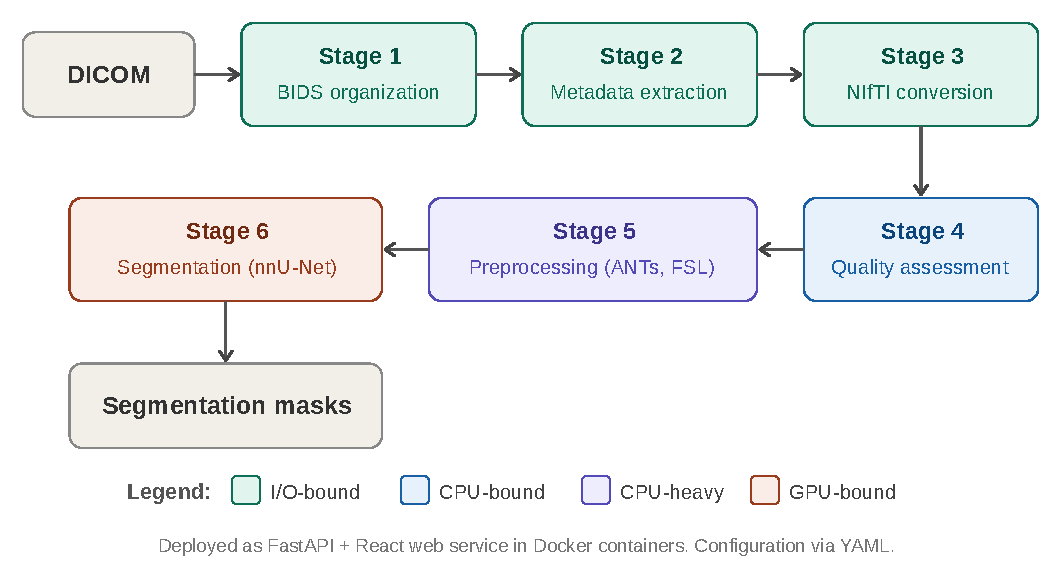
\includegraphics[width=\columnwidth]{fig1_pipeline_architecture.pdf}
\caption{Six-stage brain MRI processing pipeline. Colors indicate computational load type: green = I/O-bound, blue = CPU-bound, purple = CPU-heavy, coral = GPU-bound.}
\label{fig:pipeline}
\end{figure}

\textbf{Stage~1: BIDS Organization.} Raw Digital Imaging and Communications in Medicine (DICOM) files in an arbitrary directory structure are reorganized into the Brain Imaging Data Structure (BIDS) format~\cite{gorgolewski2016}. The system automatically detects MRI modalities (T1, T1ce, T2, FLAIR) and maps them to BIDS-compliant filenames. In this study, the input comprises 100 patients (110 imaging sessions totaling 424 MRI series, with each session containing 1--4 modalities) from the UPENN-GBM glioblastoma dataset~\cite{bakas2022}.

\textbf{Stage~2: Metadata Extraction.} Selected DICOM tags are extracted and stored separately, after which patient-identifying information is removed from the original headers.

\textbf{Stage~3: NIfTI Conversion.} DICOM series are converted to the Neuroimaging Informatics Technology Initiative (NIfTI) format using dcm2niix~\cite{li2016}.

\textbf{Stage~4: Quality Assessment.} Eight image quality metrics are computed for each volume: Signal-to-Noise Ratio (SNR), Contrast-to-Noise Ratio (CNR), Entropy Focus Criterion (EFC), Foreground--Background Energy Ratio (FBER), Gradient Sharpness, Voxel Anisotropy, Intensity Variance, and Coefficient of Variation. Values are normalized and classified into three quality grades---poor, acceptable, good---based on configurable per-modality thresholds.

\textbf{Stage~5: Preprocessing.} The most computationally intensive stage performs four sequential operations: (1)~N4 bias field correction, (2)~affine registration of the reference modality (T1 by default) to a standard brain atlas using Advanced Normalization Tools (ANTs)~\cite{avants2009}, followed by registration of remaining modalities to the aligned reference, (3)~skull stripping via the FSL Brain Extraction Tool (BET)~\cite{smith2002}, and (4)~intensity normalization.

\textbf{Stage~6: Segmentation.} Brain lesion segmentation is performed using nnU-Net~\cite{isensee2021}, chosen for its self-configuring design and established performance on brain tumor benchmarks. The model was pretrained on a multi-class brain tumor dataset~\cite{pnev2022}. Inference is executed on a configurable GPU server, supporting multi-GPU parallelization through an asynchronous client architecture with explicit CUDA device assignment. The pipeline architecture is model-agnostic: the segmentation backend can be substituted without affecting other stages.

The pipeline is deployed as a web service with a FastAPI backend and React frontend, containerized via Docker. The source code and benchmarking scripts are publicly available in the project repository \texttt{KateRoppert/mri\_ai\_service} on GitHub.

\section{Experimental Results}

\subsection{Experimental Setup}

All CPU-bound experiments (Stages~1--5) were conducted on a workstation with an Intel Core i7-13700KF processor (16 cores / 24 threads, up to 5.4~GHz), 64~GB DDR5 RAM, NVMe SSD storage, running Ubuntu 24.04 LTS. For GPU-based segmentation (Stage~6), three servers were used: \textit{Server~A} (2$\times$NVIDIA RTX A4500, 20~GB VRAM each), \textit{Server~B} (1$\times$NVIDIA Quadro RTX 8000, 48~GB VRAM), and \textit{Server~C} (1$\times$NVIDIA GeForce GTX TITAN X, 12~GB VRAM).

The dataset comprises 100 patients from the UPENN-GBM collection~\cite{bakas2022}, yielding 110 imaging sessions across four MRI modalities (T1, T1ce, T2, FLAIR). Not all sessions contain the full set of modalities: 103 sessions include the T1 reference required for preprocessing (Stage~5), and 98 sessions contain all four modalities required by the nnU-Net model for segmentation (Stage~6). For each CPU-bound stage, we varied the number of parallel processes from 1 to 20.

\subsection{Methodology}

To ensure measurement validity, we implemented a controlled benchmarking protocol. Before each experiment run, the operating system disk cache was explicitly cleared (\texttt{sync} followed by \texttt{echo 3 > /proc/sys/vm/drop\_caches}) with a 2-second stabilization delay. This step proved critical: preliminary experiments without cache clearing showed artificially inflated speedups for I/O-bound stages, with some configurations appearing 2--4$\times$ faster than their actual speed due to cached file reads. Where computationally feasible, each configuration was executed twice and results were averaged. Stages~1--3 exhibited less than 10\% variance across all configurations; Stages~4--5 were run once due to their long execution times (2+ hours per configuration).

\subsection{Parallelization Results}

Table~\ref{tab:optimal} summarizes the optimal configuration for each stage, and Fig.~\ref{fig:speedup} presents the speedup curves. The results reveal pronounced heterogeneity in scaling behavior across stages.

\begin{table}[t]
\centering
\caption{Optimal Parallel Configurations for Each Pipeline Stage. Time and Speedup are Reported at the Saturation Point (Sat.), Defined as the Lowest Process Count Beyond Which Throughput Gain is Less Than 5\%.}
\label{tab:optimal}
\begin{tabular}{clccccc}
\toprule
Stage & Name & Load & Sess. & Sat. & Time(s) & Speed. \\
\midrule
1 & BIDS Org. & I/O & 110 & 8 & 188.6 & 3.49$\times$ \\
2 & Metadata & I/O & 110 & 8 & 0.2 & 3.49$\times$ \\
3 & NIfTI Conv. & I/O+ & 110 & 8 & 35.5 & 3.79$\times$ \\
4 & Quality & CPU & 110 & 12 & 114.0 & 5.22$\times$ \\
5 & Preproc. & CPU & 103 & 6 & 1490.1 & 2.17$\times$ \\
6 & Segment. & GPU & 98 & 2GPU & 1230.3 & 1.94$\times$ \\
\bottomrule
\end{tabular}
\end{table}

\begin{figure}[t]
\centering
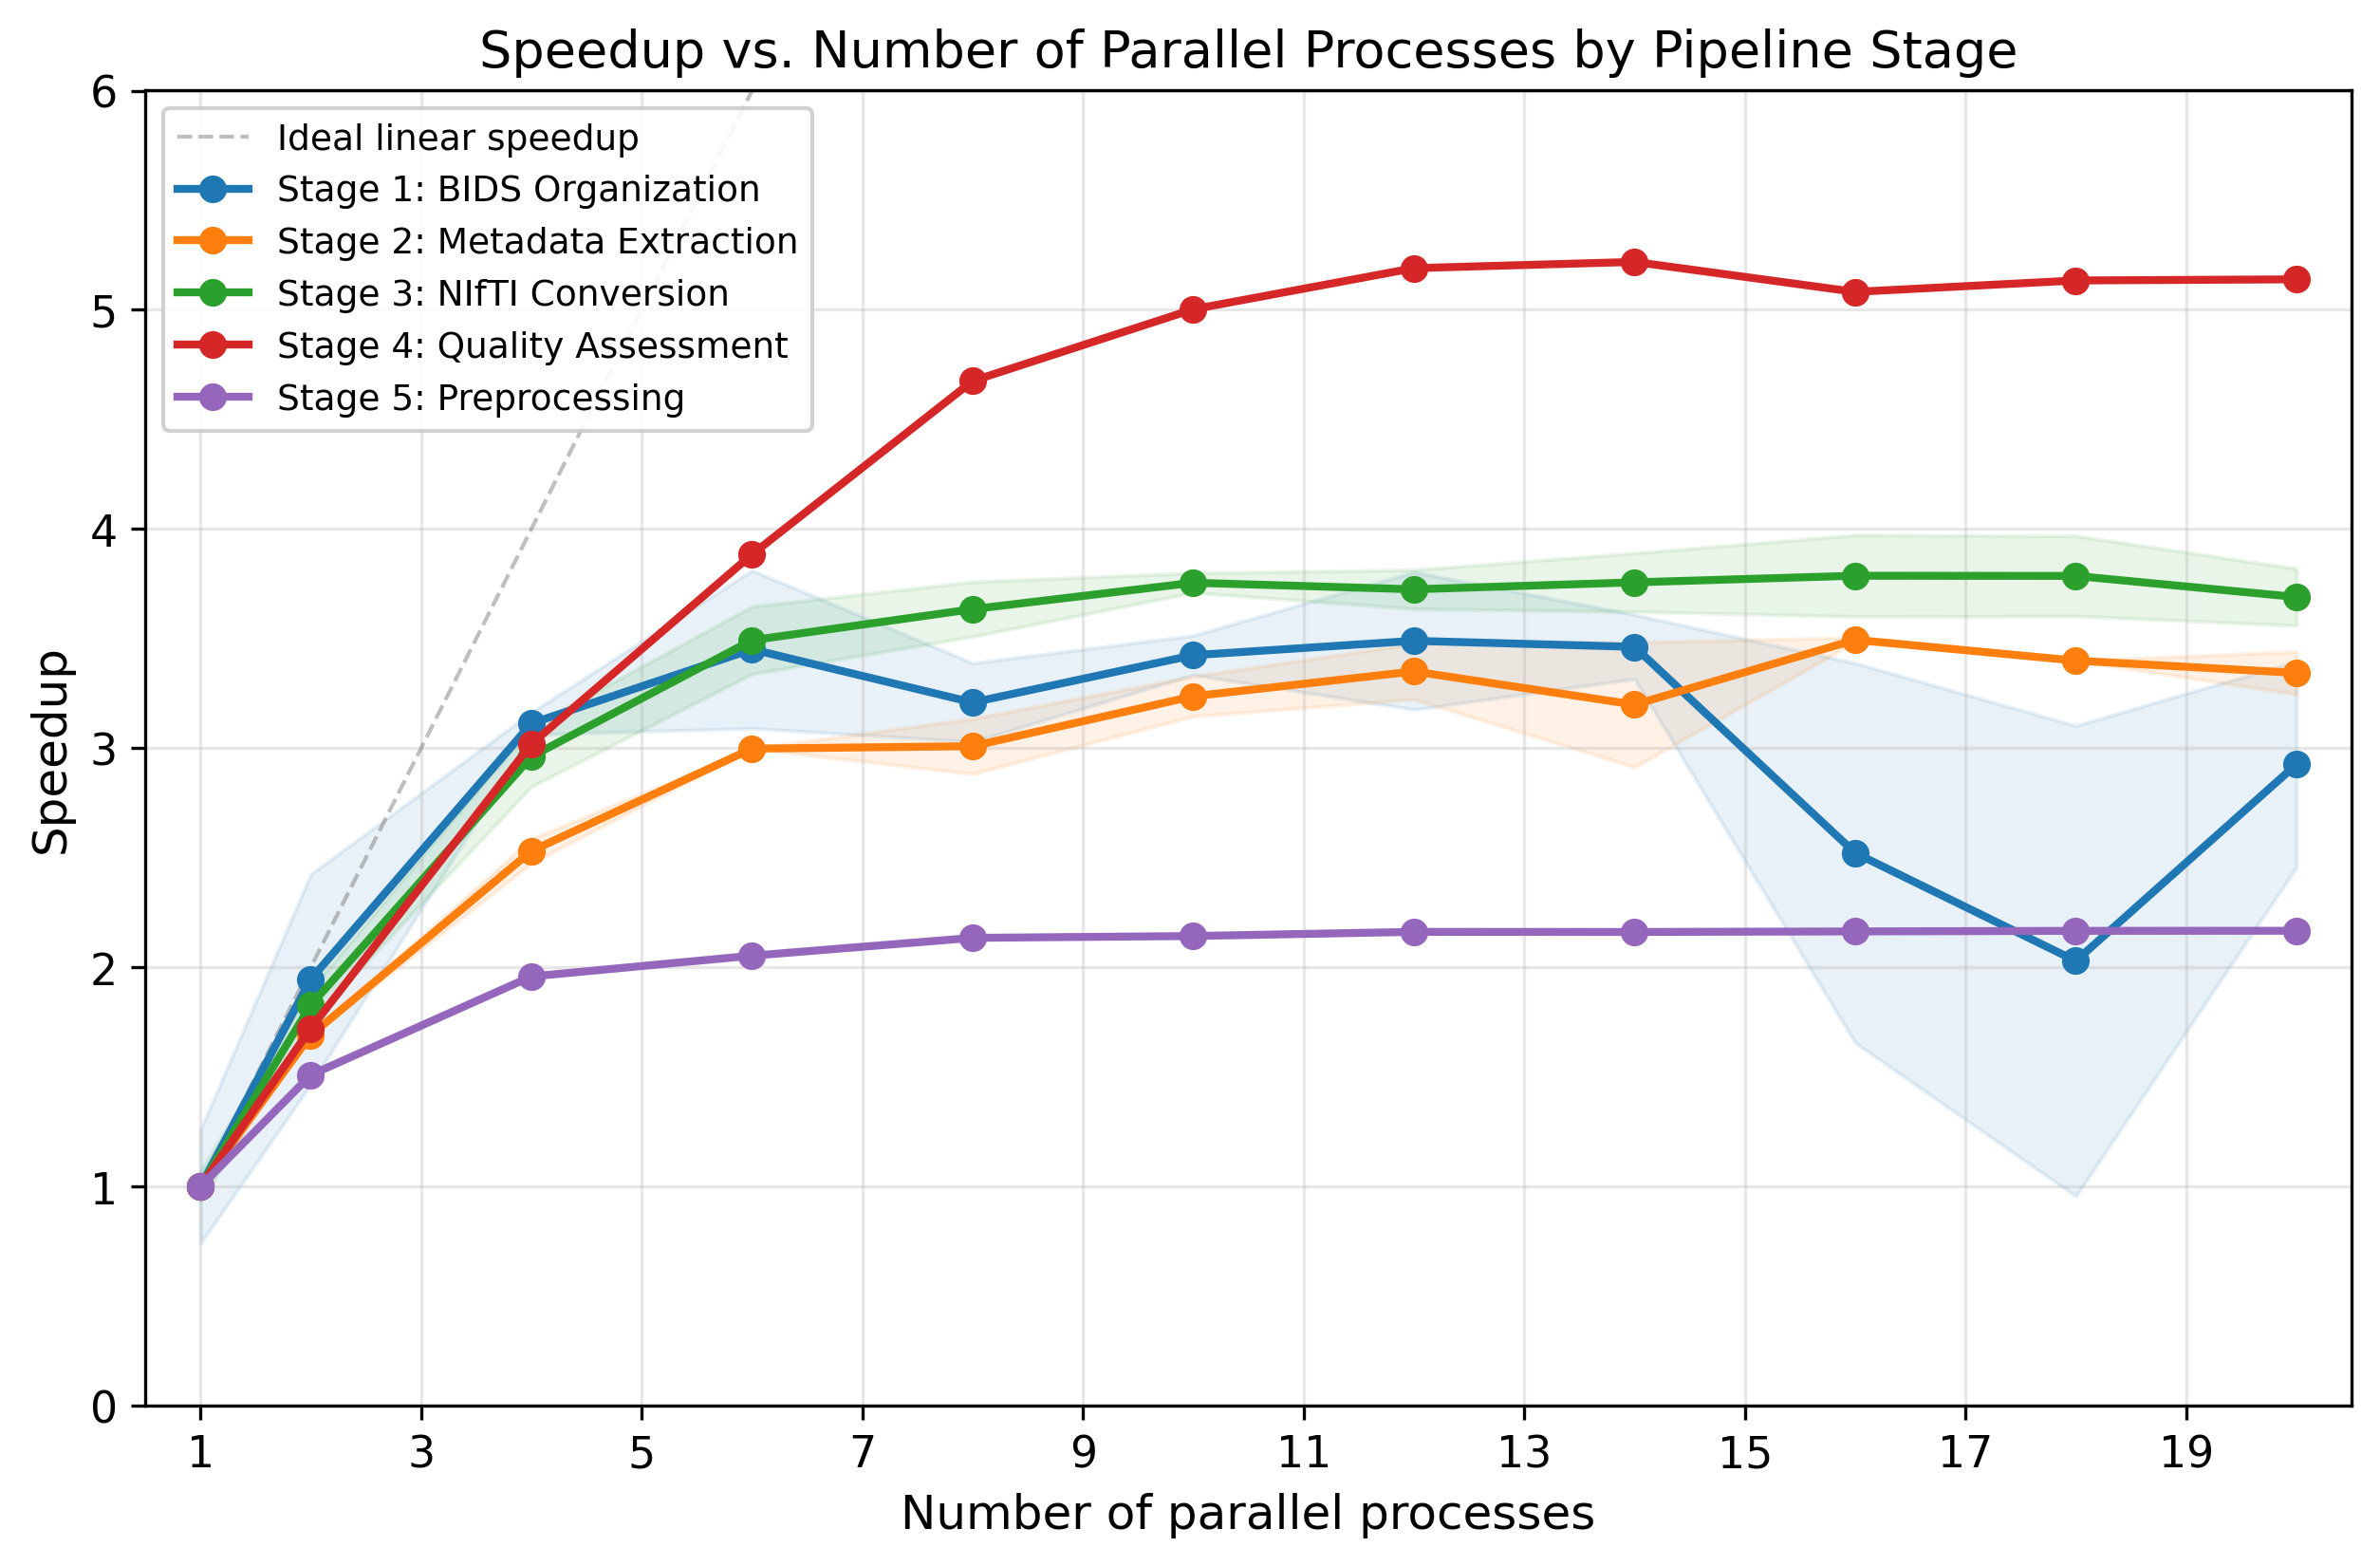
\includegraphics[width=\columnwidth]{speedup_all_stages.png}
\caption{Speedup vs.\ number of parallel processes by pipeline stage. Shaded bands indicate the range between two experimental runs. The dashed line represents ideal linear speedup.}
\label{fig:speedup}
\end{figure}

\textbf{Stages~1--3 (I/O-bound)} exhibit similar saturation at 6--8 processes with speedups of 3.5--3.8$\times$. Beyond this point, disk I/O bandwidth becomes the limiting factor. \textbf{Stage~4 (CPU-bound)} demonstrates the best scalability, achieving $5.22\times$ speedup at 12 processes with near-linear scaling up to $w = 10$. \textbf{Stage~5 (CPU-heavy)} is the most resistant to parallelization, saturating at just 6 processes with only $2.17\times$ speedup. Each preprocessing instance internally uses multiple threads for ANTs registration and FSL operations, causing CPU core contention. Memory profiling revealed that peak RAM consumption dropped from 1.7~GB at $w=1$ to 338~MB at $w \geq 2$, indicating that saturation is driven by CPU contention rather than memory exhaustion. This stage consumes 47.8\% of total pipeline time, making it the primary bottleneck. \textbf{Stage~6 (GPU-bound)} was profiled across three server configurations (Table~\ref{tab:gpu}); the dual-GPU setup on \textit{Server~A} achieves $1.94\times$ speedup with 96.8\% parallel efficiency.

\begin{table}[t]
\centering
\caption{GPU Segmentation Performance Across Servers. \textit{Server~A} Has 2~GPUs Available; Other Servers Have 1~GPU Each.}
\label{tab:gpu}
\begin{tabular}{llccc}
\toprule
Server & GPU & Used & Time/ses(s) & Speed. \\
\midrule
Server~A & 2$\times$RTX A4500 & 1 & 24.31 & 1.00$\times$ \\
Server~A & 2$\times$RTX A4500 & 2 & 12.55 & 1.94$\times$ \\
Server~B & Quadro RTX 8000 & 1 & 56.43 & 1.00$\times$ \\
Server~C & GTX TITAN X & 1 & 128.85 & 1.00$\times$ \\
\bottomrule
\end{tabular}
\end{table}

\subsection{Bottleneck Analysis}

Two stages dominate the total pipeline time: Preprocessing (47.8\%) and Segmentation (44.3\%), together accounting for 92.1\%. These percentages represent per-session processing time at each stage's individual optimal configuration and indicate the relative computational weight of each stage, not a simultaneously achievable operating point. The two dominant stages have fundamentally different resource requirements: Stage~5 is CPU- and RAM-bound, while Stage~6 is GPU-bound. This complementarity means they could execute concurrently without resource contention---an insight that motivates the MAS architecture proposed in Section~V.

\section{Proposed MAS Architecture}

The heterogeneous saturation profiles identified in Section~IV demonstrate that no single static configuration is optimal across all pipeline stages. This section proposes a MAS architecture that uses the empirical performance profiles as an operational knowledge base for dynamic resource negotiation. The primary contribution of this paper is the profiling methodology and its results; the architecture presented here is a proposed design grounded in established MAS theory, with full implementation and validation as future work.

\subsection{Agent Model}

Each Stage Manager is modeled as a Belief--Desire--Intention (BDI) agent~\cite{wooldridge1995}. \textbf{Beliefs} encode the agent's operational state: current queue depth, active process count, observed throughput, and its empirically determined saturation profile from Table~\ref{tab:optimal}. \textbf{Desires} represent the agent's objectives: minimize queue processing time while avoiding resource waste beyond the saturation point. \textbf{Intentions} are the agent's committed actions: request additional processes, release excess processes, or maintain the current allocation.

\subsection{Architecture Overview}

The system comprises three tiers. \textbf{Tier~1: Broker Agent} serves as a \textit{mediator}, not a central controller; it maintains the global resource pool, facilitates negotiation between Stage Managers, and enforces system-wide constraints. \textbf{Tier~2: Stage Manager Agents} ($\times$6) are autonomous BDI agents that independently monitor their queues, evaluate whether additional resources would improve throughput, and participate in resource negotiation through a Contract Net--inspired protocol. \textbf{Tier~3: Worker Processes} are managed computational resources allocated to Stage Managers as a result of negotiation. The architecture satisfies Wooldridge and Jennings' MAS properties~\cite{wooldridge1995}: autonomy (Stage Managers decide independently and the Broker cannot force release), reactivity (agents respond to runtime anomalies without external intervention), proactivity (agents anticipate demand and release resources before being asked), and social ability (substantive communication via the negotiation protocol).

\subsection{Resource Negotiation Protocol}

Resource allocation follows a protocol inspired by the Contract Net Protocol (CNP)~\cite{smith1980}, a foundational coordination mechanism in MAS that has been widely adopted in modern agent frameworks~\cite{dorri2018}. \textit{Step~1: Announcement.} When a Stage Manager's queue exceeds a threshold and its process count is below saturation, it issues a resource request to the Broker. \textit{Step~2: Call for bids.} The Broker broadcasts the request; other Stage Managers may offer to release processes if their queue is empty or allocation exceeds saturation. \textit{Step~3: Evaluation and award.} The Broker evaluates bids and awards resources, prioritizing release from the most over-saturated stages. This protocol preserves agent autonomy: Stage Managers decide \textit{whether} to bid and \textit{how many} processes to offer.

\section{Performance Modeling}

To quantify the benefit of dynamic resource allocation, we constructed a simulation model driven by the empirical throughput data from Section~IV. The model compares four strategies across batch sizes of 20, 50, and 100 patients, using $P = 24$ CPU processes and $G = 2$ GPU devices.

\subsection{Throughput Model}

For each CPU-bound stage $i$ with $w$ allocated processes, throughput is derived from empirical measurements:
\begin{equation}
\theta(i, w) = N_i / T(i, w),
\end{equation}
where $N_i$ is the number of sessions in the experiment and $T(i, w)$ is the measured wall time. Linear interpolation is applied for intermediate worker counts.

\subsection{Four Allocation Strategies}

\textbf{Strategy~1: Sequential.} One process, stages one after another: $M_{\text{seq}} = \sum n_i / \theta(i, 1)$.

\textbf{Strategy~2: Stage-Sequential Parallel.} Full CPU pool per stage, stages one after another (current system): $M_{\text{ss}} = \sum n_i / \theta(i, \min(P, s_i))$, where $s_i$ denotes the empirically determined saturation point of stage~$i$ (column ``Sat.'' in Table~\ref{tab:optimal}).

\textbf{Strategy~3: Pipeline Parallel.} Stages concurrent with fixed allocation $w_i$ scaled to budget $P$: $M_{\text{pip}} = \max_i \{ \text{start}(i) + n_i / \theta(i, w_i) \}$.

\textbf{Strategy~4: MAS (Dynamic).} Discrete-event simulation with initial allocation as Strategy~3, periodic reallocation every 10s, and 1s overhead per reallocation cycle.

In Strategies~3 and~4, GPU segmentation operates as part of the pipeline: it begins as soon as the first session completes preprocessing, overlapping with ongoing CPU stages. For 100 patients, this eliminates approximately 25 minutes of GPU idle time present in Strategies~1 and~2.

\subsection{Results}

Table~\ref{tab:sim} presents the simulation results, and Fig.~\ref{fig:makespan} visualizes the makespan comparison.

\begin{table}[t]
\centering
\caption{Simulation Results: Four Allocation Strategies}
\label{tab:sim}
\begin{tabular}{clcccc}
\toprule
$N$ & Strategy & Mksp. & Speed. & CPU\% & Thr \\
\midrule
\multirow{4}{*}{20}
& Sequential & 21.4 & 1.00$\times$ & 4.2 & 56 \\
& Stage-Seq. & 9.4 & 2.29$\times$ & 46.0 & 128 \\
& Pipeline & 6.6 & 3.23$\times$ & 12.4 & 181 \\
& \textbf{MAS} & \textbf{5.4} & \textbf{4.00$\times$} & \textbf{29.4} & \textbf{224} \\
\midrule
\multirow{4}{*}{50}
& Sequential & 53.3 & 1.00$\times$ & 4.2 & 56 \\
& Stage-Seq. & 23.3 & 2.29$\times$ & 45.8 & 129 \\
& Pipeline & 16.3 & 3.26$\times$ & 12.6 & 184 \\
& \textbf{MAS} & \textbf{10.9} & \textbf{4.88$\times$} & \textbf{31.9} & \textbf{274} \\
\midrule
\multirow{4}{*}{100}
& Sequential & 106.2 & 1.00$\times$ & 4.2 & 57 \\
& Stage-Seq. & 46.4 & 2.29$\times$ & 46.0 & 129 \\
& Pipeline & 32.6 & 3.26$\times$ & 12.6 & 184 \\
& \textbf{MAS} & \textbf{22.6} & \textbf{4.7$\times$} & \textbf{31.6} & \textbf{266} \\
\bottomrule
\end{tabular}\\[4pt]
\footnotesize $N$ = batch size; Mksp. = makespan (min); Thr = throughput (pat/hr).
\end{table}

\begin{figure}[t]
\centering
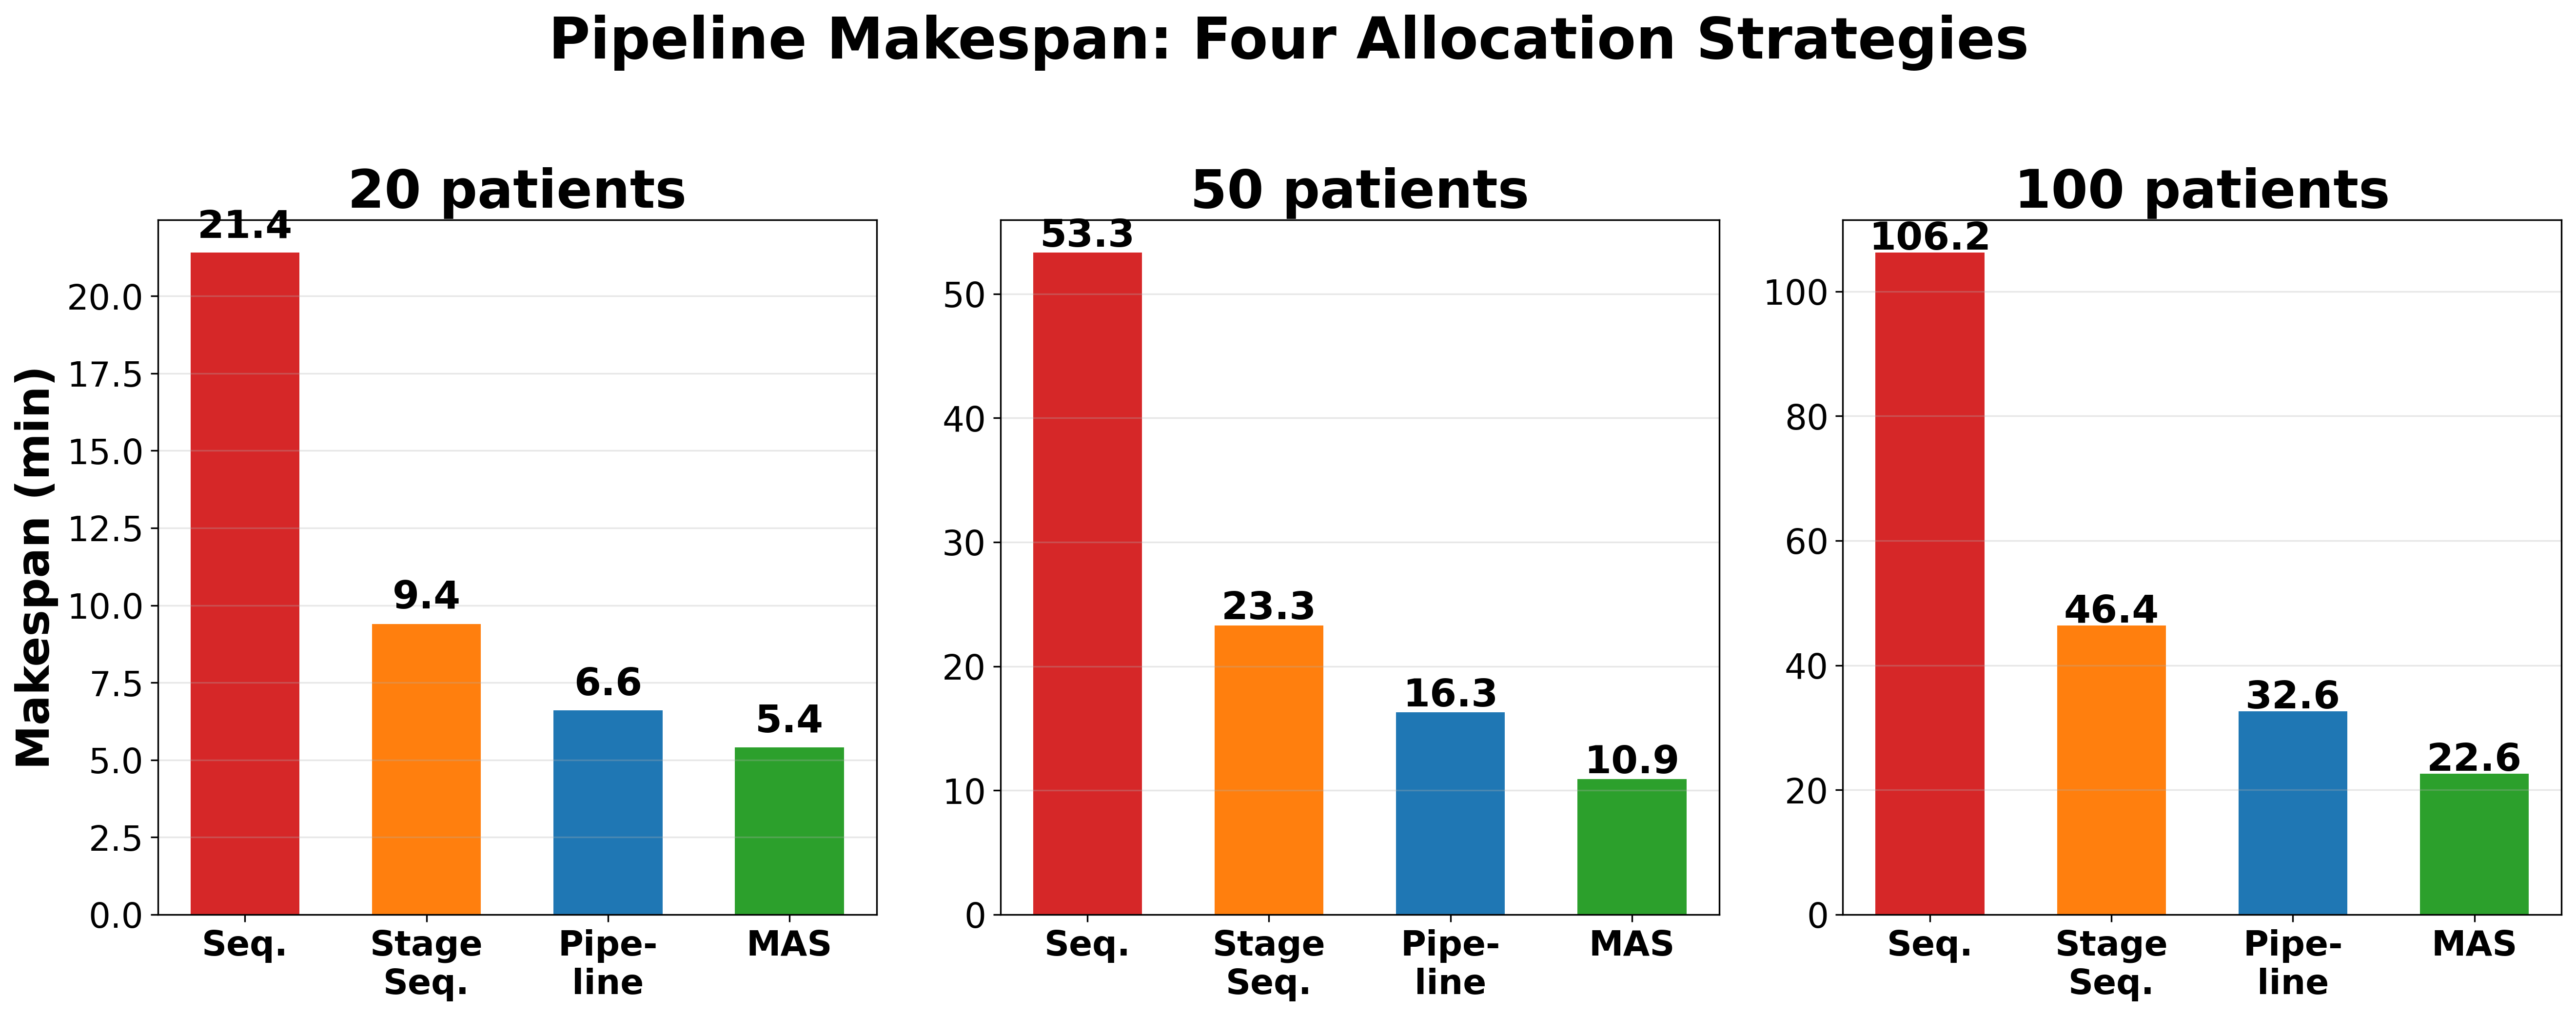
\includegraphics[width=\columnwidth]{makespan_comparison.png}
\caption{Pipeline makespan comparison across four resource allocation strategies for batch sizes of 20, 50, and 100 patients.}
\label{fig:makespan}
\end{figure}

Four findings emerge. First, pipeline overlap outweighs per-stage resource depth: Pipeline Parallel achieves $3.26\times$ speedup versus $2.29\times$ for Stage-Sequential at 100 patients, despite each stage receiving fewer processes. Second, dynamic reallocation closes the utilization gap: MAS reaches $4.7\times$ speedup at 100 patients (a 44\% improvement over Pipeline Parallel) as processes from completed early stages migrate to the Preprocessing bottleneck, which scales from 2 to 6 workers. Third, the benefit grows with batch size: MAS reduces makespan by 19\% over Pipeline at 20 patients and by 31\% at 100. Fourth, GPU overlap is critical---in MAS mode, GPU segmentation runs concurrently with preprocessing, and their throughputs nearly match (1 session per 12.5s vs 15s), yielding a balanced pipeline. The MAS advantage is also robust to negotiation overhead: at 100 patients (${\sim}20$ reallocation cycles), raising per-cycle overhead from 1s to 10s only increases makespan from 22.6 to 25.6~min, still 21\% faster than Pipeline Parallel.

\section{Discussion}

\subsection{MAS vs.\ Parallelism}

The gains could in principle be achieved by a dynamic scheduler without multi-agent concepts, and the simulation in Section~VI models the effect of dynamic reallocation as a principle rather than the specific overhead of multi-agent negotiation. Three architectural distinctions nonetheless justify the MAS approach: \textit{decentralized knowledge} (each Stage Manager encapsulates its own saturation profile as a local belief, so adding a new pipeline stage requires only deploying a new agent); \textit{negotiation rather than dictation} (the CNP-based protocol allows agents to refuse resource release based on local state, handling runtime deviations from the empirical model); and \textit{proactive behavior} (agents anticipate demand and release resources before being asked, reducing effective reallocation latency). These advantages---decentralized knowledge management, fault tolerance through agent autonomy, and modular extensibility---become critical in multi-node clinical deployments not captured by a single-machine simulation.

Existing cluster schedulers such as YARN, Kubernetes, and Slurm operate at the container or node level and allocate resources based on declared requirements, not on empirical stage-specific saturation profiles. They cannot express the constraint ``Stage~5 gains nothing beyond 6~processes while Stage~4 scales to~12'' without manual configuration that must be updated whenever the pipeline, hardware, or dataset changes. The proposed MAS internalizes these profiles as agent beliefs, enabling automatic adaptation---a capability that general-purpose schedulers lack by design.

\subsection{Clinical Applicability}

Current clinical workflows process MRI studies sequentially. Even with optimal static parallelization, 100 studies require 46 minutes. The MAS-based pipeline reduces this to 23 minutes and produces results incrementally: based on the simulation trace, the first segmentation result becomes available within minutes of pipeline start, enabling a \textit{streaming} clinical workflow. The profiling methodology is reusable: a new site would run the benchmarking script, obtain its own saturation profiles, and configure the MAS agents accordingly.

\subsection{Limitations}

The MAS architecture and performance model have been evaluated through simulation only, not through a deployed prototype; consequently, real-world communication overhead and process migration costs remain to be measured. The simulation assumes deterministic per-session throughput derived from batch averages, while real clinical data exhibit per-patient variability in image size, resolution, and modality completeness that may shift saturation points and affect reallocation timing. All empirical data derive from the UPENN-GBM glioblastoma dataset with multi-modal 3D MRI; saturation profiles may differ substantially for other pathologies (e.g., multiple sclerosis with smaller lesion loads), single-modality protocols, or datasets of significantly different size. The 1-second reallocation overhead is an optimistic estimate, and GPU segmentation accounts for ${\sim}80\%$ of MAS makespan---further improvement requires additional GPU resources.

\section{Conclusion}

This paper addressed resource management in multi-stage brain MRI processing pipelines through empirical profiling, architectural design, and simulation-based evaluation. A six-stage pipeline was benchmarked under a controlled cache-clearing protocol, revealing stage-specific saturation points (6--12 processes) and showing that preprocessing and segmentation account for 92\% of pipeline time. The resulting empirical saturation points and throughput curves serve directly as BDI agent beliefs, bridging systems benchmarking and multi-agent architecture design, and motivate a three-tier MAS (Broker, Stage Managers, Workers) with Contract Net--inspired negotiation. In simulation, this MAS achieves $4.7\times$ speedup over sequential processing at 100 patients, outperforming both stage-sequential ($2.29\times$) and pipeline parallelism ($3.26\times$); GPU/CPU overlap and dynamic resource migration are the primary mechanisms driving the advantage. Future work will proceed along three directions. First, a prototype MAS will be implemented using the SPADE agent framework within the existing FastAPI/Docker infrastructure; key metrics to be measured include inter-agent message latency, negotiation convergence time, and process migration overhead, enabling direct comparison between simulated and empirical MAS performance. Second, the profiling study will be replicated on additional datasets---including MS60 for multiple sclerosis lesion segmentation---to assess how saturation profiles vary across pathologies and imaging protocols. Third, the agent model will be extended to support multi-node distributed deployment with heterogeneous GPU resources across clinical sites, where the decentralization advantages of MAS over centralized schedulers are expected to be most pronounced.

\section*{Acknowledgment}

This work was supported by a grant for research centers, provided by the Ministry of Economic Development of the Russian Federation in accordance with the subsidy agreement with the Novosibirsk State University dated April 17, 2025 No.~139-15-2025-006: IGK 000000C313925P3S0002.

\begin{thebibliography}{20}
\bibitem{isensee2021} F. Isensee, P.~F. Jaeger, S.~A.~A. Kohl, J. Petersen, and K.~H. Maier-Hein, ``nnU-Net: a self-configuring method for deep learning-based biomedical image segmentation,'' \textit{Nature Methods}, vol.~18, no.~2, pp.~203--211, 2021, doi: 10.1038/s41592-020-01008-z.

\bibitem{wooldridge2009} M. Wooldridge, \textit{An Introduction to MultiAgent Systems}, 2nd~ed. Chichester, U.K.: Wiley, 2009, pp.~1--461, ISBN: 978-0-470-51946-2.

\bibitem{wooldridge1995} M. Wooldridge and N.~R. Jennings, ``Intelligent agents: Theory and practice,'' \textit{The Knowledge Engineering Review}, vol.~10, no.~2, pp.~115--152, 1995, doi: 10.1017/S0269888900008122.

\bibitem{tang2024} X. Tang, A. Zou, Z. Zhang, Z. Li, Y. Zhao, X. Zhang, A. Cohan, and M. Gerstein, ``MedAgents: Large language models as collaborators for zero-shot medical reasoning,'' in \textit{Findings of the Association for Computational Linguistics: ACL 2024}, Bangkok, Thailand, 2024, pp.~599--621, doi: 10.18653/v1/2024.findings-acl.33.

\bibitem{kim2024} Y. Kim, C. Park, H. Jeong, Y.~S. Chan, X. Xu, D. McDuff, H. Lee, M. Ghassemi, C. Breazeal, and H.~W. Park, ``MDAgents: An adaptive collaboration of LLMs for medical decision-making,'' in \textit{Advances in Neural Information Processing Systems 37 (NeurIPS 2024)}, Vancouver, Canada, 2024, pp.~1--26, doi: 10.48550/arXiv.2404.15155.

\bibitem{zhu2025} K. Zhu, Y. Yang, H. Wang, Z. Wu, J. Wang, and B. Xu, ``MedAgentBoard: Benchmarking multi-agent collaboration with conventional methods for diverse medical tasks,'' in \textit{Proc. 39th Conf. Neural Information Processing Systems (NeurIPS 2025) Datasets and Benchmarks Track}, 2025, pp.~1--32, doi: 10.48550/arXiv.2505.12371.

\bibitem{kirimtat2024} A. Kirimtat and O. Krejcar, ``GPU-based parallel processing techniques for enhanced brain magnetic resonance imaging analysis: A review of recent advances,'' \textit{Sensors}, vol.~24, no.~5, p.~1591, 2024, doi: 10.3390/s24051591.

\bibitem{hashisho2024} M.~M. Hashisho, S.~M. Awad, A.~M. Hassanien, and N.~M. Mahmoud, ``High performance computing for image processing on medical field: Parallelization techniques,'' \textit{International Journal of Computer Science and Information Security (IJCSIS)}, vol.~22, no.~3, pp.~78--90, 2024.

\bibitem{smistad2019} E. Smistad, A. Ostvik, and L. Lovstakken, ``High performance neural network inference, streaming, and visualization of medical images using FAST,'' \textit{IEEE Access}, vol.~7, pp.~136486--136496, 2019, doi: 10.1109/ACCESS.2019.2942441.

\bibitem{predescu2024} M. Predescu, X. Yang, M. Jones, D. Rogers, and B.~A. Landman, ``High-throughput computing: Case study of medical image processing applications,'' in \textit{Proc. 14th Workshop on AI and Scientific Computing at Scale using Flexible Computing (FlexScience'24)}, Pisa, Italy: ACM, 2024, pp.~1--8, doi: 10.1145/3659994.3660313.

\bibitem{wang2025} Z. Wang, H. Wang, J. Liu, Y. Zhao, and L. Zhou, ``MedAgent-Pro: Towards multi-modal evidence-based medical diagnosis via reasoning agentic workflow,'' in \textit{Proc. 42nd International Conference on Machine Learning (ICML 2025)}, Vienna, Austria, 2025, pp.~1--18, doi: 10.48550/arXiv.2503.18968.

\bibitem{yang2026} C. Yang, F. Wang, R. Zhang, K. Liu, and J. Chen, ``LungNoduleAgent: A collaborative multi-agent system for automated lung nodule diagnosis from CT imaging,'' in \textit{Proc. AAAI Conf. on Artificial Intelligence}, vol.~40, 2026, pp.~1--9, doi: 10.48550/arXiv.2511.21042.

\bibitem{gorgolewski2016} K.~J. Gorgolewski, T. Auer, V.~D. Calhoun, R.~C. Craddock, S. Das, E.~P. Duff, G. Flandin, S.~S. Ghosh, T. Glatard, Y.~O. Halchenko, D.~A. Handwerker, M. Hanke, D. Keator, X. Li, Z. Michael, C. Maumet, B.~N. Nichols, T.~E. Nichols, J. Pellman, J.~B. Poline, A. Rokem, G. Schaefer, V. Sochat, W. Triplett, J.~A. Turner, G. Varoquaux, and R.~A. Poldrack, ``The brain imaging data structure, a format for organizing and describing outputs of neuroimaging experiments,'' \textit{Scientific Data}, vol.~3, p.~160044, 2016, doi: 10.1038/sdata.2016.44.

\bibitem{bakas2022} S. Bakas, C. Sako, H. Akbari, M. Bilello, A. Sotiras, G. Shukla, J.~D. Rudie, N.~F. Santamaria, A.~F. Kazerooni, S. Pati, et~al., ``The University of Pennsylvania glioblastoma (UPenn-GBM) cohort: advanced MRI, clinical, genomics, \& radiomics,'' \textit{Scientific Data}, vol.~9, no.~1, p.~453, 2022, doi: 10.1038/s41597-022-01560-7.

\bibitem{li2016} X. Li, P.~S. Morgan, J. Ashburner, J. Smith, and C. Rorden, ``The first step for neuroimaging data analysis: DICOM to NIfTI conversion,'' \textit{Journal of Neuroscience Methods}, vol.~264, pp.~47--56, 2016, doi: 10.1016/j.jneumeth.2016.03.001.

\bibitem{avants2009} B.~B. Avants, N. Tustison, and G. Song, ``Advanced normalization tools (ANTS),'' \textit{Insight Journal}, vol.~2, no.~365, pp.~1--35, 2009, doi: 10.54294/uvnhin.

\bibitem{smith2002} S.~M. Smith, ``Fast robust automated brain extraction,'' \textit{Human Brain Mapping}, vol.~17, no.~3, pp.~143--155, 2002, doi: 10.1002/hbm.10062.

\bibitem{pnev2022} S. Pnev, V. Groza, B. Tuchinov, E. Amelina, E. Pavlovskiy, N. Tolstokulakov, M. Amelin, S. Golushko, and A. Letyagin, ``Multi-class brain tumor segmentation via 3D and 2D neural networks,'' in \textit{Brainlesion: Glioma, Multiple Sclerosis, Stroke and Traumatic Brain Injuries (BrainLes 2021), Lecture Notes in Computer Science}, vol.~12962. Cham: Springer, 2022, pp.~322--332, doi: 10.1007/978-3-031-08999-2\_27.

\bibitem{smith1980} R.~G. Smith, ``The Contract Net Protocol: High-level communication and control in a distributed problem solver,'' \textit{IEEE Transactions on Computers}, vol.~C-29, no.~12, pp.~1104--1113, 1980, doi: 10.1109/TC.1980.1675516.

\bibitem{dorri2018} A. Dorri, S.~S. Kanhere, and R. Jurdak, ``Multi-agent systems: A survey,'' \textit{IEEE Access}, vol.~6, pp.~28573--28593, 2018, doi: 10.1109/ACCESS.2018.2831228.
\end{thebibliography}

\end{document}